\chapter{Application User Interface }

\label{Chapter6_appUI} 

\begin{comment}
-------------------------------------------------
%								Chapter layout
6. Application User Interface 
	a. Main Layout
		b. User Specific Data Collection
		c. Visual Rotation of Gesture
	d. Tabular Display of Data
	e. Writing and Reading from CSV
	f. Artifacts and Distribution
		i. Leap App Store
		ii. IDE Build Process and Batch Script
-------------------------------------------------
figures needed:

homescreen,
analyze screen.
load folder button clicked. opened dialog. 
save to csv opened dialog
load/create new user screen. 
load/create new user screen. (with dropdown showing)
testing screen
testing screen after rotation done. also showing user hand. 



table with editing in progress. 

\end{comment}


In this chapter some of the useful UI features of the application will be discussed. 

%------------------------------------------------
%	SECTION 0 Main Layout
%------------------------------------------------
\section{Main Layout}

The application has three main scenes. One is the home screen which shows buttons to take the user to the other two scenes. It also contains two radio buttons to allow the user to select which hand (left or right) he/she will be testing with the gestures. Figure  \ref{fig:homeScreen} shows the layout of the home screen. 
\begin{figure}[H]
\centering
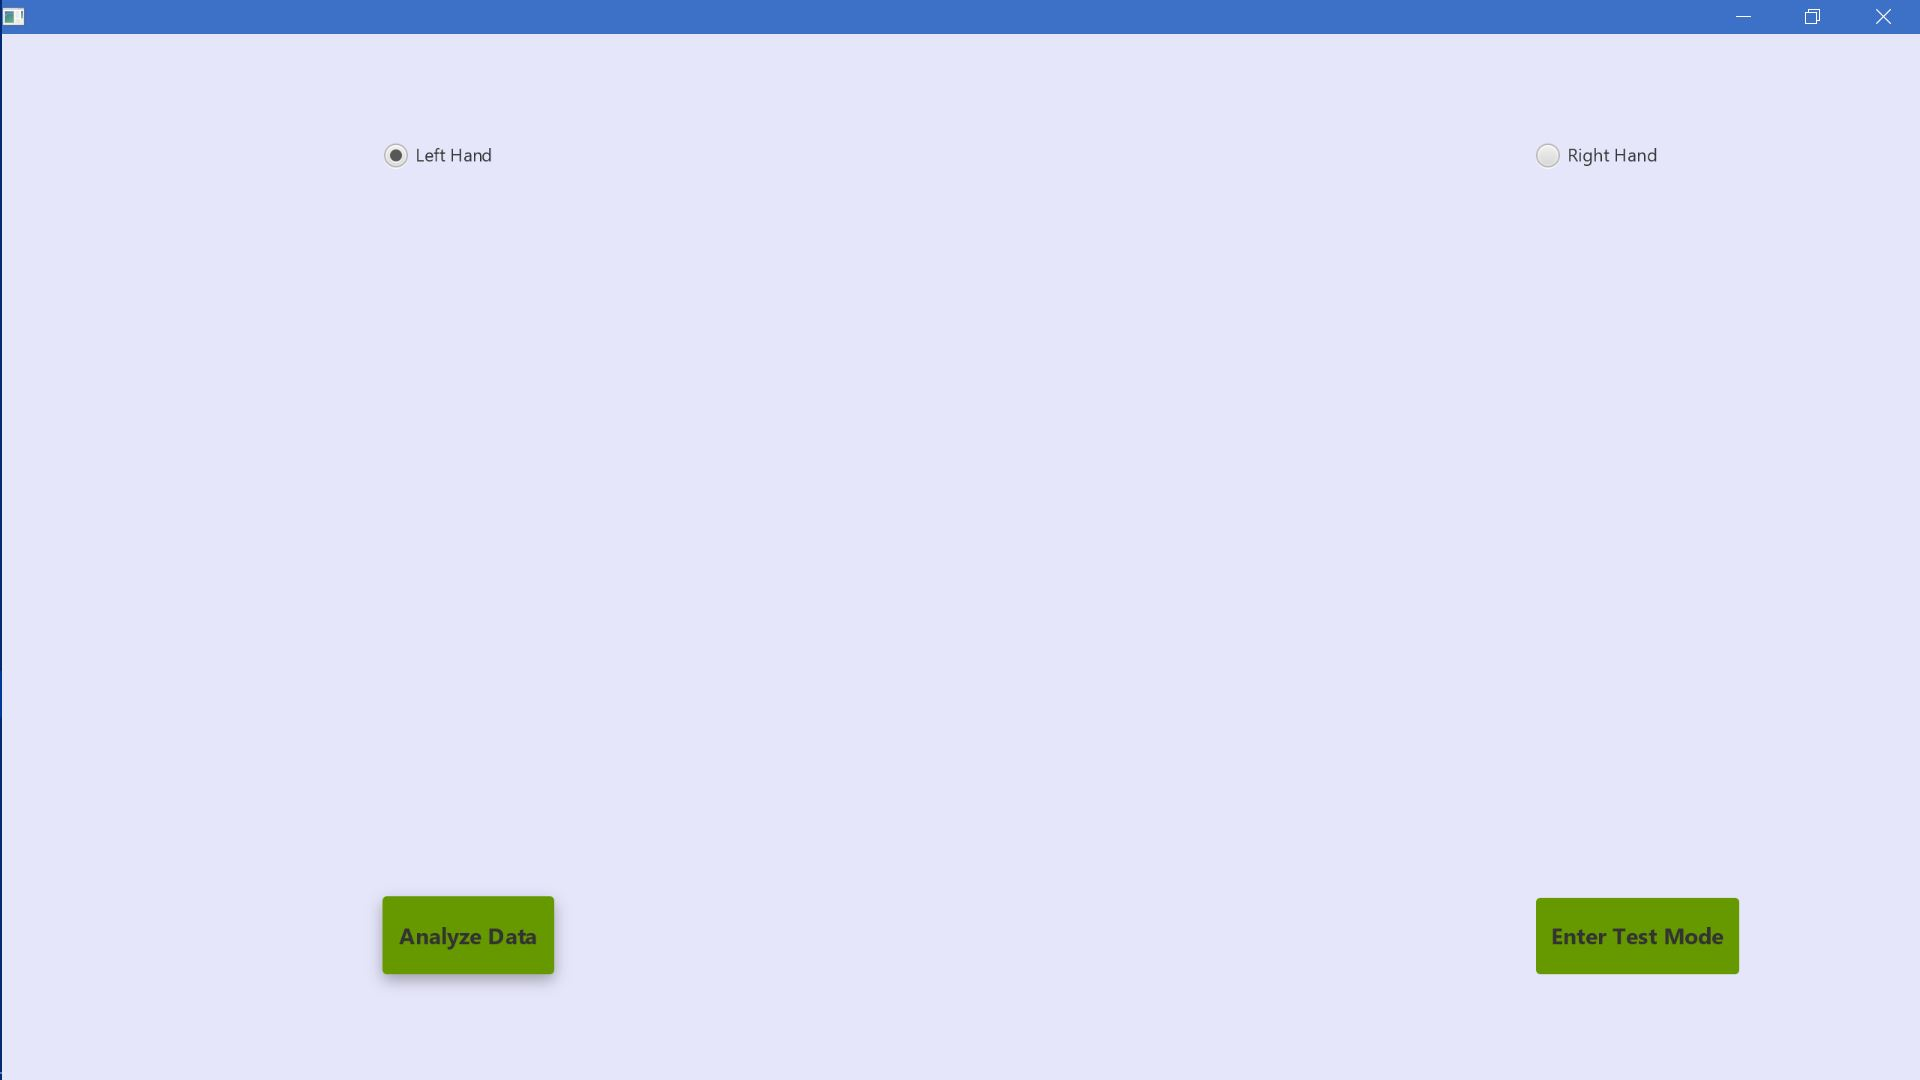
\includegraphics[scale=0.35]{Figures/6_homeScreen.JPG}
\caption[Home Screen Layout]{The scene that the user sees initially when they load the application.}
\label{fig:homeScreen}
\end{figure}

The user can click on the "Enter Test Mode" to go to the scene where data will be collected. However, before the user can go to the data collection scene, they must first select a previously saved user or create a new user. All of the hand gesture data collected will be stored in an appropriately named folder for the user. Therefore, when the user clicks on the "Enter Test Mode" the first thing that comes up is a small pop-up screen that asks whether the user would like to create a new user or select an older user; see Figure \ref{fig:createNewUser} and Figure \ref{fig:selectOldUser}. 
\begin{figure}[H]
    \centering
    \begin{minipage}{0.45\textwidth}
        \centering
        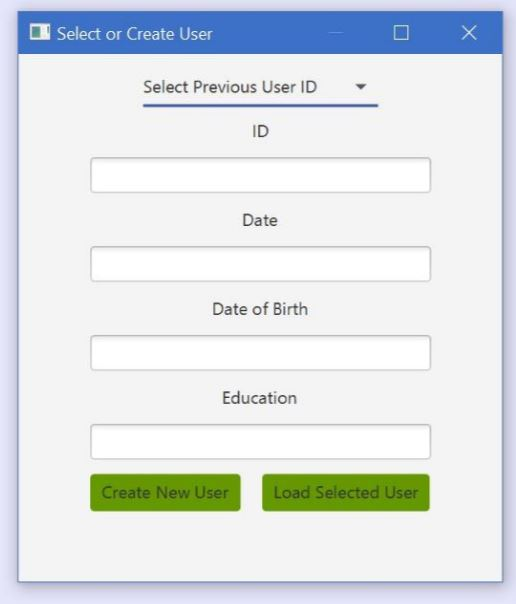
\includegraphics[scale=.45]{Figures/6_selectUser.JPG} 
        \caption{Pop-up window showing options to create or select user. }
		\label{fig:createNewUser}
    \end{minipage}\hfill
    \begin{minipage}{0.45\textwidth}
        \centering
        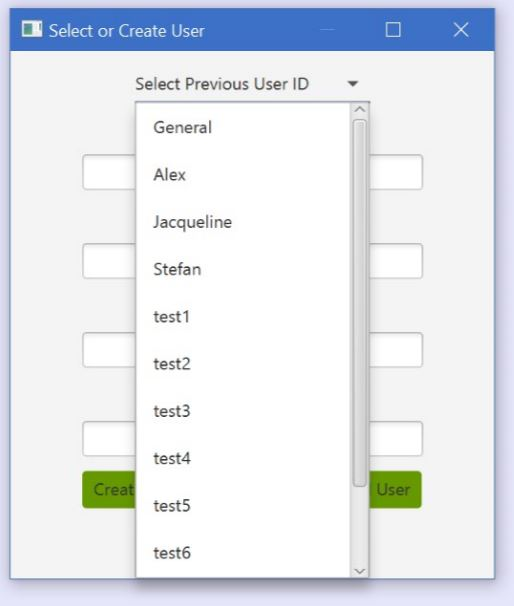
\includegraphics[scale=.45]{Figures/6_selectUserDropdown.JPG}%note png, lower case
        \caption{Pop-up window showing the previously created users.}
        \label{fig:selectOldUser}
    \end{minipage}
\end{figure}

After having created or selected a user, the user is taken to the screen where he/she can start to proceed to practicing the ten gestures shown for whichever left/right hand was selected on the home screen; see Figure \ref{fig:dataCollectionScreen}. On this data collection screen there are five buttons; Next and Previous load the cycle through the 

user hand is blue, target hand is green. dont have to be on top of the target hand to get a higher score. 

rotation button spins both hands (this will be discussed in subsection reference or name.)
displayed in a full 360 circle in 7 seconds. at this slow speed the user is able to get a feel for the orientation of their hand the gesture is perdicting. it is sometimes better to see the rotation before attempting. though the user can keep his hand.. and the hand will be spun around also. note














 which is designed for the user to go through the ten target gestures for the selected hand




 The user can click on the "Analyze Data" button to go to the 


talk about three scenes and show pics. show what happens where and 
what the typical user would do. 
take data and analyze it for problems. 
and then go fix those problems. 
also save data to csv. read from csv. 
say some things will be dicussed in other sections. 


%------------------------------------------------
%	SECTION 1 User Specific Data Collection
%------------------------------------------------
\section{User Specific Data Collection}


show the 2 figures. explain why you needed ot make users. meeting with clinicians. working product demonstration. agile. as opposed ot waterfall (this should go in conclusion). 

 

%------------------------------------------------
%	SECTION 2 Visual Rotation of Gesture
%------------------------------------------------
\section{Visual Rotation of Gesture}

same as above. 

%------------------------------------------------
%	SECTION 3 Tabular Display of Data
%------------------------------------------------
\section{Tabular Display of Data}

editable picture. show code. 
%------------------------------------------------
%	SECTION 4 Writing and Reading from CSV
%------------------------------------------------
\section{Writing and Reading from CSV}


%------------------------------------------------
%	SECTION 5 Artifacts and Distribution
%------------------------------------------------
\section{Artifacts and Distribution}

%----------------------------------- Leap App Store
\subsection{Leap App Store}

%----------------------------------- IDE Build Process and Batch Script
\subsection{IDE Build Process and Batch Script}


